
\section{Formal definition of \lsystem}

\lsystem $L$ is formally triplet $L = (\Sigma, \omega, R)$, where

\begin{itemize*}
	\item $\Sigma$ is \emph{alphabet}, non-empty set of symbols, $\Sigma^{*}$ is set of all words\footnote{Word is a sequence of symbols.} which can be created from the alphabet $\Sigma$, $\Sigma^{+}$ is set of all non-empty words which can be created from the the alphabet $\Sigma$,
	\item $\omega \in \Sigma^{+}$ is \emph{axiom} (also called seed), word defining the initial state of the \lsystem,
	\item $R \subset \Sigma \times \Sigma^{*}$ is finite set of \emph{rewrite rules} (production rules), rewrite rule defining rewriting symbol $s \in \Sigma$ to word $w \in \Sigma^{*}$ is written as $s \rightarrow w$.
\end{itemize*}

For any symbol $s \in \Sigma$ which does not appear on the left hand side of any rewrite rule in $R$, the identity rewrite rule $s \rightarrow s$ is assumed.
These symbols are called constants or terminals.

Formal definition of \lsystem is similar to deterministic context-free grammar but there are few differences.
In grammar we distinguishes terminal and non-terminal symbols, but in \lsystems we do not define them explicitly (we define identity rewrite rule for terminal symbols in \lsystems).
Next difference is in initial string.
In grammar we have only one symbol as initial state but \lsystem allows non-empty word.
The biggest difference is in rewriting principles which is described is following section.


\subsection{Rewriting principles of \lsystem}

Starting with axiom (0th iteration) in each iteration \emph{all} symbols are rewritten with rewrite rules forming next iteration.
All symbols can be rewritten because every symbol is on the left side of some rewrite rule.
% (if symbol have not been on the left side of some rewrite rule, identity rule would be defined).
There is only one way how to rewrite symbols in iteration thus rewriting is deterministic, result depends only on axiom.

Rewriting of symbols is parallel (all symbols are rewritten at once).
This means that if some symbol is rewritten, resulting symbols are not rewritten again in the same iteration.

Described rewriting principles distinguishes \lsystem and formal grammar.
In grammar there is not mandatory to rewrite all possible symbols (derivation of start state can result in more different derivations).
Thus, \lsystems are strict subsets of languages.

\lsystem \ref{lsys:rrExample} produces strings shown in Table \ref{fig:rrExampleResult}.
\lsystem starts with axiom $A$ and two rewrite rules $A \rightarrow B$ and $B \rightarrow A, B$.
In the first iteration axiom $A$ is rewritten by first rewrite rule to $B$.
In the second iteration is $B$ rewritten with second rewrite rule to symbols $A, B$.
In the third iteration is first symbol $A$ rewritten to $B$ and second symbol $B$ rewritten to $A, B$ which gives string $B, A, B$ and so on.

\begin{Lsystem}[label=lsys:rrExample,caption={Simple \lsystem as example of rewriting principles}]
lsystem RewritingExample {
	set symbols axiom = A;
	set iterations = 6;
	set interpretEveryIteration = true;
	@rewrite A to B;@
	@rewrite B to A B;@
}
process all with SymbolPrinter;
\end{Lsystem}

\begin{table}[h]
	\centering
	\begin{tabular}{c l}
   		\toprule
   		Iteration & String of symbols \\
   		\midrule
		0 & A \\
		1 & B \\
		2 & A B \\
		3 & B A B \\
		4 & A B B A B \\
		5 & B A B A B B A B \\
		6 & A B B A B B A B A B B A B \\
		\bottomrule
	\end{tabular}
	\caption{Result of \lsystem \ref{lsys:rrExample}}
	\label{fig:rrExampleResult}
\end{table}


\subsection{Interpretation of \lsystem symbols}

Result of \lsystem rewriting is string of symbols.
As it was mentioned in the \nameref{sec:Introduction} we can interpret string of symbols in any way for example as computer graphics or music.

The most common and the simplest interpretation of \lsystem symbols is interpret them as 2D graphics elements like lines or polygons.
This interpretation is often called \emph{turtle graphics} and it will be used in the most \lsystems in this thesis.
This approach can be easily extended into 3D.

Let symbol \texttt{F} is interpreted as \emph{draw line forward}, \texttt{+} as \emph{turn left} and \texttt{-} as turn right.
Figure \ref{fig:intSequences} shows interpreted strings of symbols.
Initial direction is to the right.

\begin{figure}[h]
	\centering
	\subfloat[\texttt{F + F - - F + F}, turning angle: $60^{\circ}$]{
		
\includegraphics[scale=1]{IntTriangle}
	} ~
	\subfloat[\texttt{F + F - F - F + F}, turning angle: $90^{\circ}$]{
		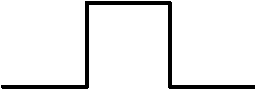
\includegraphics[scale=1]{IntSquare}
	} ~
	\subfloat[\texttt{F + F + + F - F - - F F - F}, turning angle: $60^{\circ}$]{
		\hspace{9mm}
\includegraphics[scale=1]{IntHexa}\hspace{9mm}
	}
	\caption{Examples of interpretation simple string of symbols}
	\label{fig:intSequences}
\end{figure}


More complex string of symbols as an example of interpretation is generated by \lsystem in Source code \ref{lsys:intExampleCode} where symbol $F$ is interpreted as \emph{draw line forward}, symbol $+$ is interpreted as \emph{turn left} by 85 degrees and symbol $-$ as \emph{turn right} by 85 degrees (equally as \emph{turn left} by $-85$ degrees).
Result of interpretation of the first, second and fourth iteration is in Figure \ref{fig:intExample}.

\begin{Lsystem}[label=lsys:intExampleCode,caption={Symbol interpretation example}]
lsystem InterpretationExample {
	set symbols axiom = F;
	set iterations = 4;
	@interpret F as DrawForward(10);@
	@interpret + as TurnLeft(85);@
	@interpret - as TurnLeft(-85);@
	rewrite F to F + F - - F + F;
}
process all with SvgRenderer;
\end{Lsystem}

\begin{figure}[h]
	\centering
	\subfloat{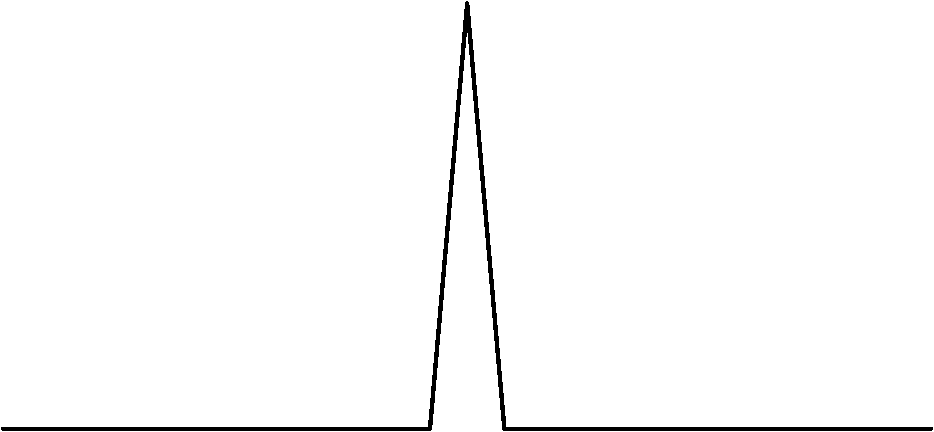
\includegraphics[width=0.3\textwidth]{Interpretation1}} ~
	\subfloat{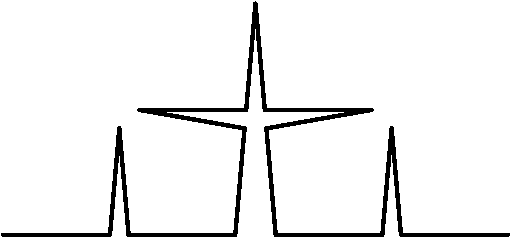
\includegraphics[width=0.3\textwidth]{Interpretation2}} ~
	\subfloat{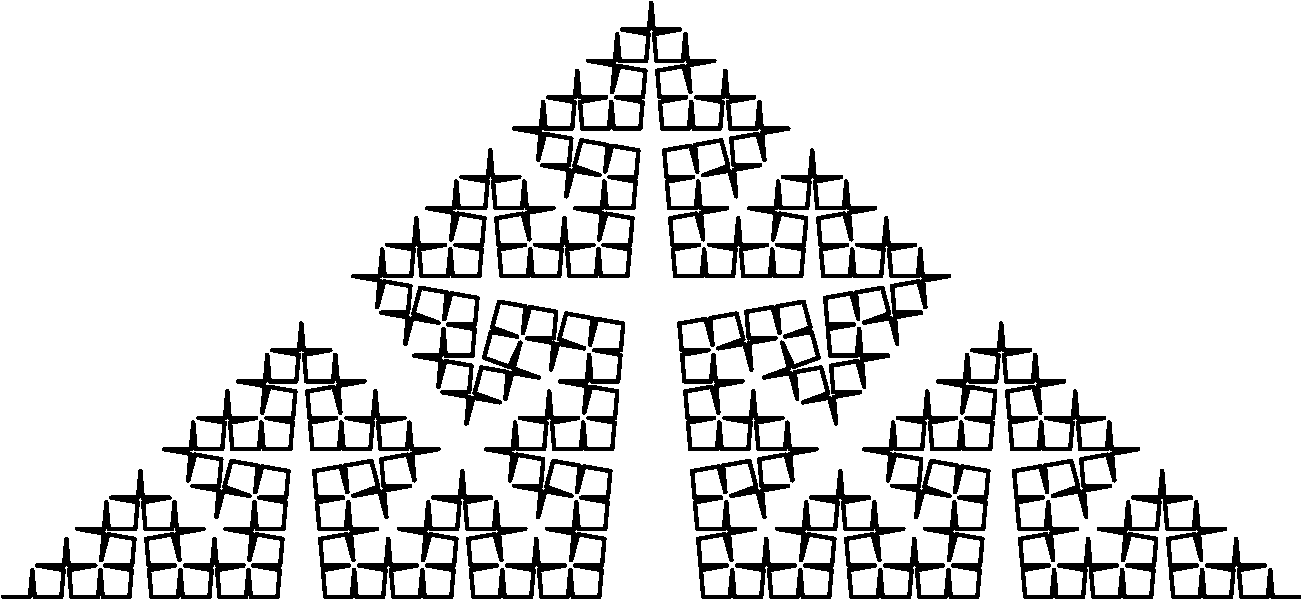
\includegraphics[width=0.3\textwidth]{Interpretation3}}
	\caption{The first, second and fourth iteration of Cesaro curve \lsystem \ref{lsys:intExampleCode}}
	\label{fig:intExample}
\end{figure}

\newpage
\section{\lsystem types}

In this section we will describe different types of \lsystems.
Some types may require extension of described formal definition of \lsystem but it will be omitted.

\lsystems described so far are called \emph{deterministic \lsystems} because their rewriting system is deterministic.
\emph{Bracketed \lsystems} allows to save and load state of interpretation.
This can be used to model branches of plants more easily.
\emph{Stochastic \lsystems} can randomize result model to suppress its artificiality.
\emph{Context-sensitive \lsystems} allows to rewrite symbol depending on its context (symbols around it).
Symbols in \emph{parametric \lsystems} can hols any number of arguments which can be used while rewriting or interpreting symbol.

Any of described types can be combined together.



\subsection{Deterministic \lsystems}

\newcommand{\dzerolsystem}{\mbox{D0L-system}\xspace}
\newcommand{\dlsystem}{\mbox{dL-system}\xspace}


\begin{wrapfigure}{r}{0.50\textwidth}
	\vspace{-40pt}
	\begin{center}
	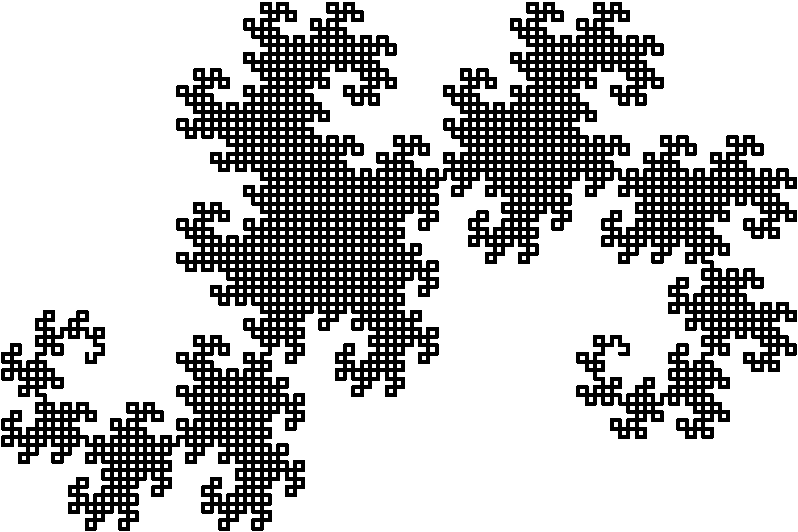
\includegraphics[width=0.48\textwidth]{BasicLsystem}
	\end{center}
	\caption{Dragon curve}
	\label{fig:basicLsystem}
\end{wrapfigure}


Basic \lsystem type described by previous formal definition is called \dzerolsystem\footnote{\dzerolsystem is also called just \dlsystem~\cite{Zar04}.}.
\emph{D} means that rewriting is deterministic and \emph{0} means it is context-free.
The result of \dzerolsystem depends only on initial string of symbols.

This type of \lsystem is often used to generate fractal curves.
By using \dzerolsystem \ref{fig:basicLsystem} we can generate Dragon curve that you can see in Fig. \ref{lsys:basicLsystemSrc}.

\begin{Lsystem}[label=lsys:basicLsystemSrc,caption={Basic \dzerolsystem for generation of Dragon curve (Fig. \ref{fig:basicLsystem})}]
lsystem DragonCurve {
	set symbols axiom = L;
	set iterations = 12;
	interpret R L as DrawForward(5);
	interpret + as TurnLeft(90);
	interpret - as TurnLeft(-90);
	rewrite L to L + R +;
	rewrite R to - L - R;
}
process all with SvgRenderer;
\end{Lsystem}


\subsection{Bracketed \lsystems}

First and important extension to \dzerolsystem is branching system.
This type of \lsystem is called Bracketed \lsystem\cite{PL91}.
Branching is so fundamental feature that Bracketed \lsystems are often called just \lsystems.

Branching system extends symbol interpretation by two commands \emph{start branch} and \emph{end branch}.
These commands are nearly always represented as symbols of brackets (from which bracketed \lsystems got their name).
Open bracket "\texttt{[}" as start branch and close bracket "\texttt{]}" as close branch.

Start branch command saves the state of interpretation which can be loaded by end branch command later.
In turtle graphics interpretation state is position, orientation and drawing color of turtle.
More than one states can be saved at the same time, last saved state will be loaded first.
This behavior is natural and could be compared to pairing of brackets.

Branching extends linear string of symbols to the tree structure.
Individual branches do not affect each other nor their root.
This allows to model plants more easily and create more complex models.

Bracketed \lsystem \ref{lsys:branchingSrc} demonstrates usage of branching system to produce plant-like model which you can see in Figure \ref{fig:branching}.
Note that color of segments indicates their type and age.
Brown segments are drawn with symbol \texttt{F} and they represent segments from previous iteration.
Green segments are drawn with symbol \texttt{A} and they are new compared to the previous iteration.

\begin{Lsystem}[label=lsys:branchingSrc,caption={Bracketed \lsystem which creates plant-like model (Fig. \ref{fig:branching})}]
lsystem PythagorasTree {
	set symbols axiom = A;
	set initialAngle = 90;
	set iterations = 4;	
	interpret A F as DrawForward(16);
	interpret + as TurnLeft(45);
	interpret - as TurnLeft(-45);
	@interpret [ as StartBranch;@
	@interpret ] as EndBranch;@
	rewrite A to F [ + A ] [ - A ] F A;
	rewrite F to F F;
}
process all with SvgRenderer;
\end{Lsystem}

\begin{figure}[h]
	\centering
	\subfloat{
\includegraphics[scale=1]{Branching1}} ~
	\subfloat{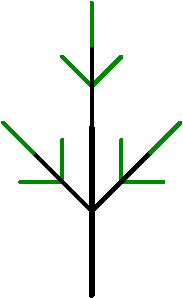
\includegraphics[scale=1]{Branching2}} ~
	\subfloat{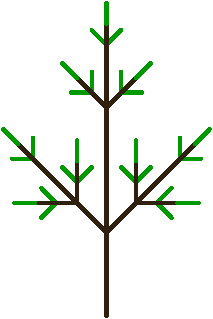
\includegraphics[scale=1]{Branching3}} ~
	\subfloat{
\includegraphics[scale=1]{Branching4}}
	\caption{First four iterations of bracketed \lsystem \ref{lsys:branchingSrc}}
	\label{fig:branching}
\end{figure}



\subsection{Stochastic \lsystems}

\newcommand{\zerolsystem}{\mbox{0L-system}\xspace}
\newcommand{\zerolsystems}{\mbox{0L-systems}\xspace}

All plants generated by same deterministic \lsystem are identical.
Forest made by trees which are identical looks artificial and can not be used in films or video games.
Stochastic \lsystems solves this problem because they can produce randomized model.
Stochastic \lsystems are called \zerolsystem where 0 means they are context-free.

Randomization of model produced by \lsystem can be done in two places, in rewrite rules or in interpretation of symbols (or in both).
Randomization in interpretation can only change properties of interpreted symbols such as lengths of lines or turning angles, the topology of plant remains unchanged.
In contrast with rewrite rule randomization which can also change topology of model.
Rewrite rule randomization is done by defining more replacements for one rewrite rule.
Rewriting system will pick random replacement if rewrite rule is applied.
Each replacement can have different probability to be picked.

In Figure \ref{fig:randComparison} are shown 3 models of plant generated by stochastic \lsystems.
First image \ref{fig:randComparisonNo} was generated without any randomization.
Second image \ref{fig:randComparisonInt} was generated with interpretation randomization of line lengths and angles.
For last image \ref{fig:randComparisonBoth} was also added topology randomization with rewrite rule randomization (Source code \ref{lsys:randExample}).

\begin{figure}[h]
	\centering
	\subfloat[No randomization]{
		\label{fig:randComparisonNo}
		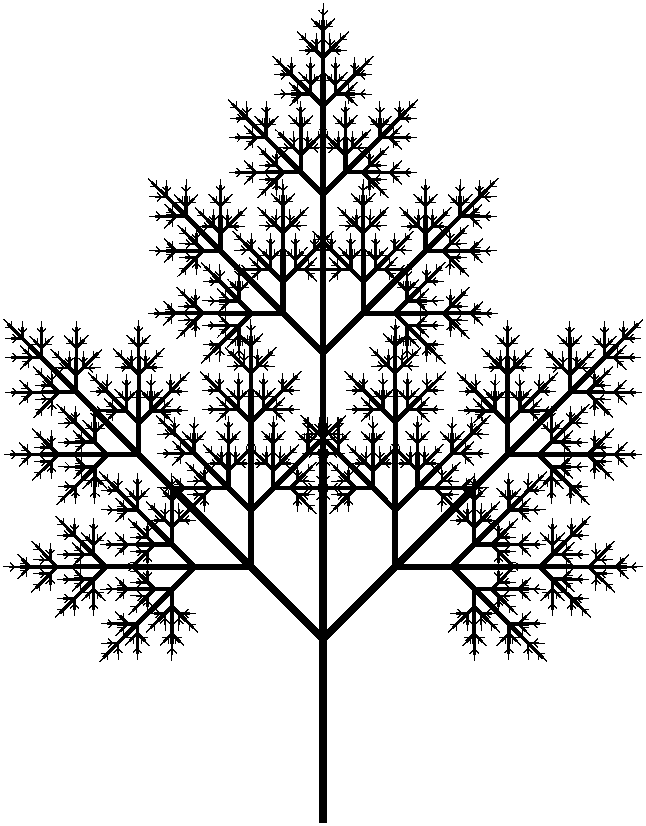
\includegraphics[width=0.3\textwidth]{StochasticLsystemExample-NoStochasism}
	} ~
	\subfloat[Angles, lengths randomized]{
		\label{fig:randComparisonInt}
		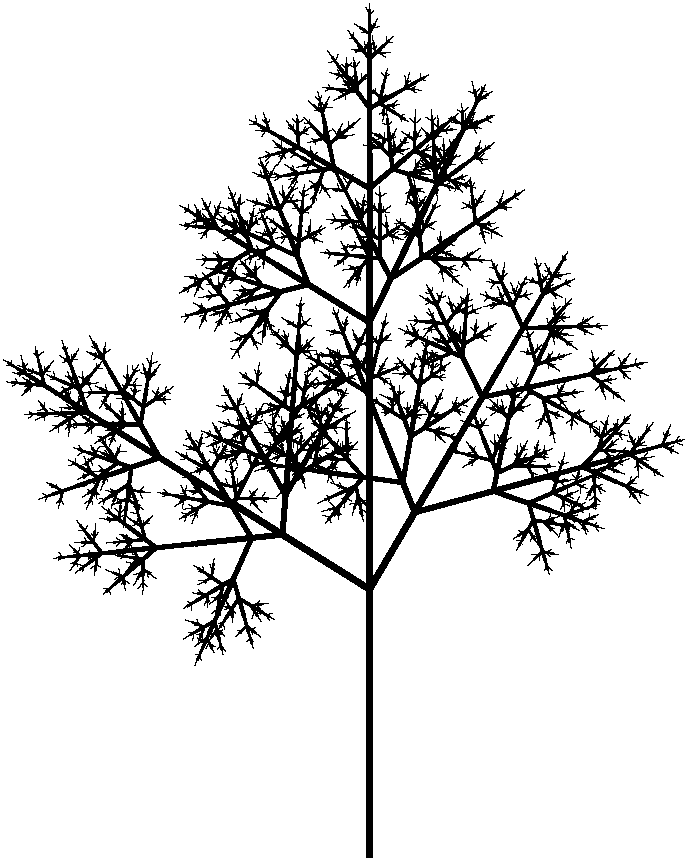
\includegraphics[width=0.32\textwidth]{StochasticLsystemExample-InterpretationStochasism}
	} ~
	\subfloat[Also topology randomized]{
		~
		\label{fig:randComparisonBoth}
		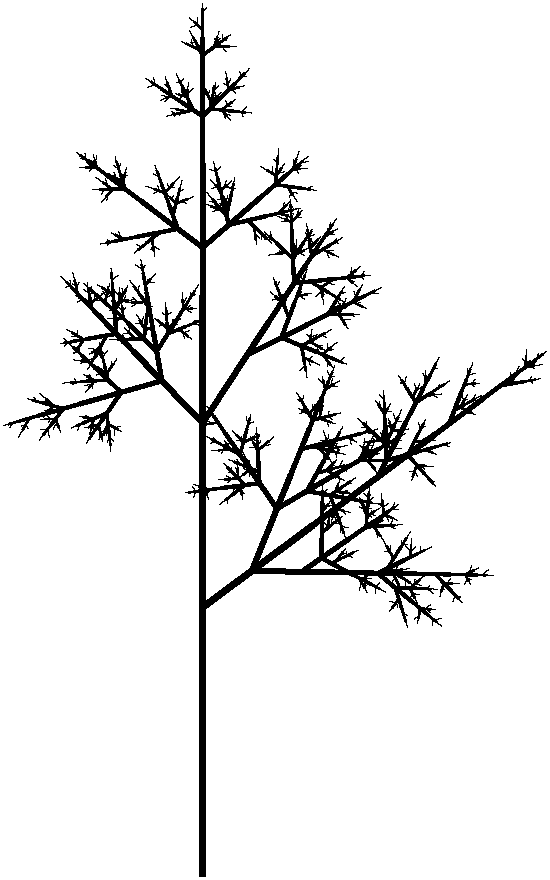
\includegraphics[width=0.25\textwidth]{StochasticLsystemExample-BothStochasism}
		~
	}
	\caption{Comparison between non-randomized and randomized plant model}
	\label{fig:randComparison}
\end{figure}

\begin{Lsystem}[label=lsys:randExample,caption={Example of stochastic \lsystem with randomized rewrite rules and interpretation}]
lsystem StochasticLsystemExample {
	set symbols axiom = X;
	set initialAngle = 90;
	set iterations = 8;
	set randomSeed = 1036793868;

	interpret F(age) as DrawForward(1.8^age*random(0.5,1.5), age/2);
	interpret + as TurnLeft(45 + random(-20, 20));
	interpret - as TurnLeft(-45 + random(-20, 20));
	interpret [ as StartBranch;
	interpret ] as EndBranch;

	rewrite F(age) to F(age + 1);
	@rewrite X@
		@to F(1) [ + X ] [ - X ] F(1) X  weight 4 or@
		@to F(1) [ + X ]         F(1) X  weight 1 or@
		@to F(1)         [ - X ] F(1) X  weight 1;@
}
process all with SvgRenderer;
\end{Lsystem}


\subsection{Context-sensitive \lsystems}

\newcommand{\onelsystems}{\mbox{1L-systems}\xspace}
\newcommand{\twolsystems}{\mbox{2L-systems}\xspace}

Rewriting of symbols in \zerolsystems is context-free, rewrite rules are applied on the symbols regrades of their context (symbols around it).
However rewriting of symbol can also depend on its context.
This is useful in simulating the flow of signals (nutrients or hormones) in plant model~\citep{PL91}.

Formally there are two types of context sensitive L-systems, \onelsystems and \twolsystems.
Rewrite rules of \onelsystems checks context only on one side (left or right) whereas rewrite rules of \twolsystems checks context on both sides.
Since \onelsystems are just \twolsystems with one context empty we will consider context sensitive \lsystems as \twolsystems.

Context sensitive \lsystem \ref{lsys:signalPropagarionSrc} shows simulation of signal propagation in the string of symbols.
Result is in Table \ref{fig:signalPropagarion}.

\begin{Lsystem}[label=lsys:signalPropagarionSrc,caption={Context-sensitive \lsystems simulating signal propagation}]
lsystem RewritingExample {
	set symbols axiom = B A A A A A;
	set iterations = 6;
	set interpretEveryIteration = true;
	@rewrite {B} A     to B;@
	@rewrite     B {A} to A;@
}
process all with SymbolPrinter;
\end{Lsystem}

\begin{table}[h]
	\centering
	\begin{tabular}{c l}
   		\toprule
   		Iteration & String of symbols \\
   		\midrule
		0 & B A A A A A \\
		1 & A B A A A A \\
		2 & A A B A A A \\
		3 & A A A B A A \\
		4 & A A A A B A \\
		5 & A A A A A B \\
		6 & A A A A A A \\
		\bottomrule
	\end{tabular}
	\caption{Axiom and first 6 iterations of \lsystem \ref{lsys:signalPropagarionSrc} showing signal propagation in the string of symbols}
	\label{fig:signalPropagarion}
\end{table}


\subsubsection{Context-sensitive bracketed \lsystems}

If we add context-sensitive rewrite rule to bracketed \lsystems situation will be more difficult.
The context matching procedure must take into account branches.
Following rules defines natural behavior of context between branches:
\begin{enumerate*}
	\item \label{enum:ctxRule1} two symbols are neighbors even if there are some branches between them,
	\item \label{enum:ctxRule2} left neighbor of first symbol in branch is symbol before branch,
	\item \label{enum:ctxRule3} last symbol in branch do not have right neighbor,
	\item \label{enum:ctxRule4} unmatched symbols at the end of branch are ignored,
	\item \label{enum:ctxRule5} order of branches is insignificant.
\end{enumerate*}

Table \ref{tbl:bracketCtxt} shows examples of context matching in bracketed \lsystems with references to according rules.

\begin{table}[h]
	\centering
	\begin{tabular}{c c c p{128pt} c c}
   		\toprule
   		Left ctx. & Symbol & Right ctx. & Symbol string & Match & Rule\\
   		\midrule
		 & X & Y & A B \textbf{X} [ A [ B ] ] [ C ] \textbf{Y} & yes & \ref{enum:ctxRule1} \\
		 & X & Y & A B \textbf{X} [ Y B ] C Y & no &  \\
		 Y & X & & A B \textbf{Y} [ \textbf{X} A B ] C & yes & \ref{enum:ctxRule2} \\
		 Y & X & & A B \textbf{Y} [ [ \textbf{X} A ] B ] C & yes & \ref{enum:ctxRule2} \\
		 & X & Y & A [ B \textbf{X} ] Y & no & \ref{enum:ctxRule3} \\
		 & X & [ Y ] & A B \textbf{X} [ \textbf{Y} A B ] A  & yes & \ref{enum:ctxRule4} \\
		 & X & [ [ Y ] ] & A B \textbf{X} [ [ \textbf{Y} A B ] C ] & yes & \ref{enum:ctxRule4} \\
		 & X & [ Y ] & A B \textbf{X} [ A B ] [ \textbf{Y} ] A  & yes & \ref{enum:ctxRule5} \\
		 & X & [ Y ] [ Z ] & A B \textbf{X} [ \textbf{Z} ] [ \textbf{Y} ] A  & yes & \ref{enum:ctxRule5} \\
		\bottomrule
	\end{tabular}
	\caption{Examples of context matching in bracketed \lsystems}
	\label{tbl:bracketCtxt}
\end{table}

Context in bracketed \lsystems can be used for propagation of signals through tree structure.
There are two basic types of signals.
First is \emph{acropetal} signal which spreads from root to branches and second is \emph{basipetal} which spreads in other way i.e. from branches to root.
This can be used well in plant modeling.

Figure \ref{fig:signalPropagation} shows simulation of acropetal (\ref{fig:acropetalSignal}) and basipetal (\ref{fig:basipetalSignal}) signals in static plant-like structure.
Each figure shows first 5 iterations and segments with signal are marked bolder.

\begin{figure}[h!]
	\centering
	\subfloat[Acropetal signal propagation]{
		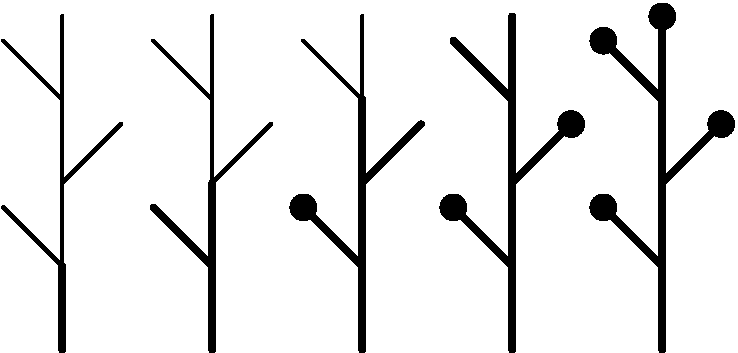
\includegraphics[scale=0.55]{AcropetalSignal}
		\label{fig:acropetalSignal}
	}
	\hspace{2mm}
	\subfloat[Basipetal signal propagation]{
		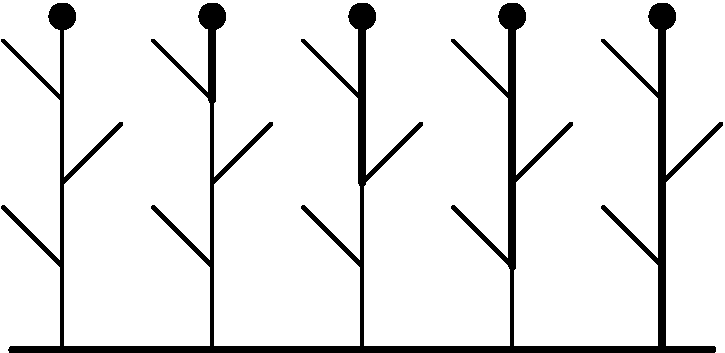
\includegraphics[scale=0.55]{BasipetalSignal}
		\label{fig:basipetalSignal}
	}
	\caption{Signal propagation simulated with context-sensitive bracketed \lsystems}
	\label{fig:signalPropagation}
\end{figure}


\subsection{Parametric \lsystems}

Symbols in parametric \lsystems can hold any number of arguments.
Arguments are often floating point numbers but they can be more complicated structures.
Arguments can be used in interpretation definition to send values like length of line or color to interpretation routine.
Arguments can be also used in rewrite rules to determine whether rewrite symbol or not and to determine new arguments for rewritten symbols.
In context \twolsystems is also possible to get arguments from symbols in context and use them in rewrite rules.




































